
\subsection{Diseño}

\begin{itemize}
  \item \textbf{Diagrama Entidad - Relación:}

  En la figura \ref{fig:er_ways}, se observa el diagrama Entidad - Relación correspondiente a los \emph{caminos} o mapa de rutas dentro del campus Universitario.


\begin{figure}[H]
  \begin{center}
    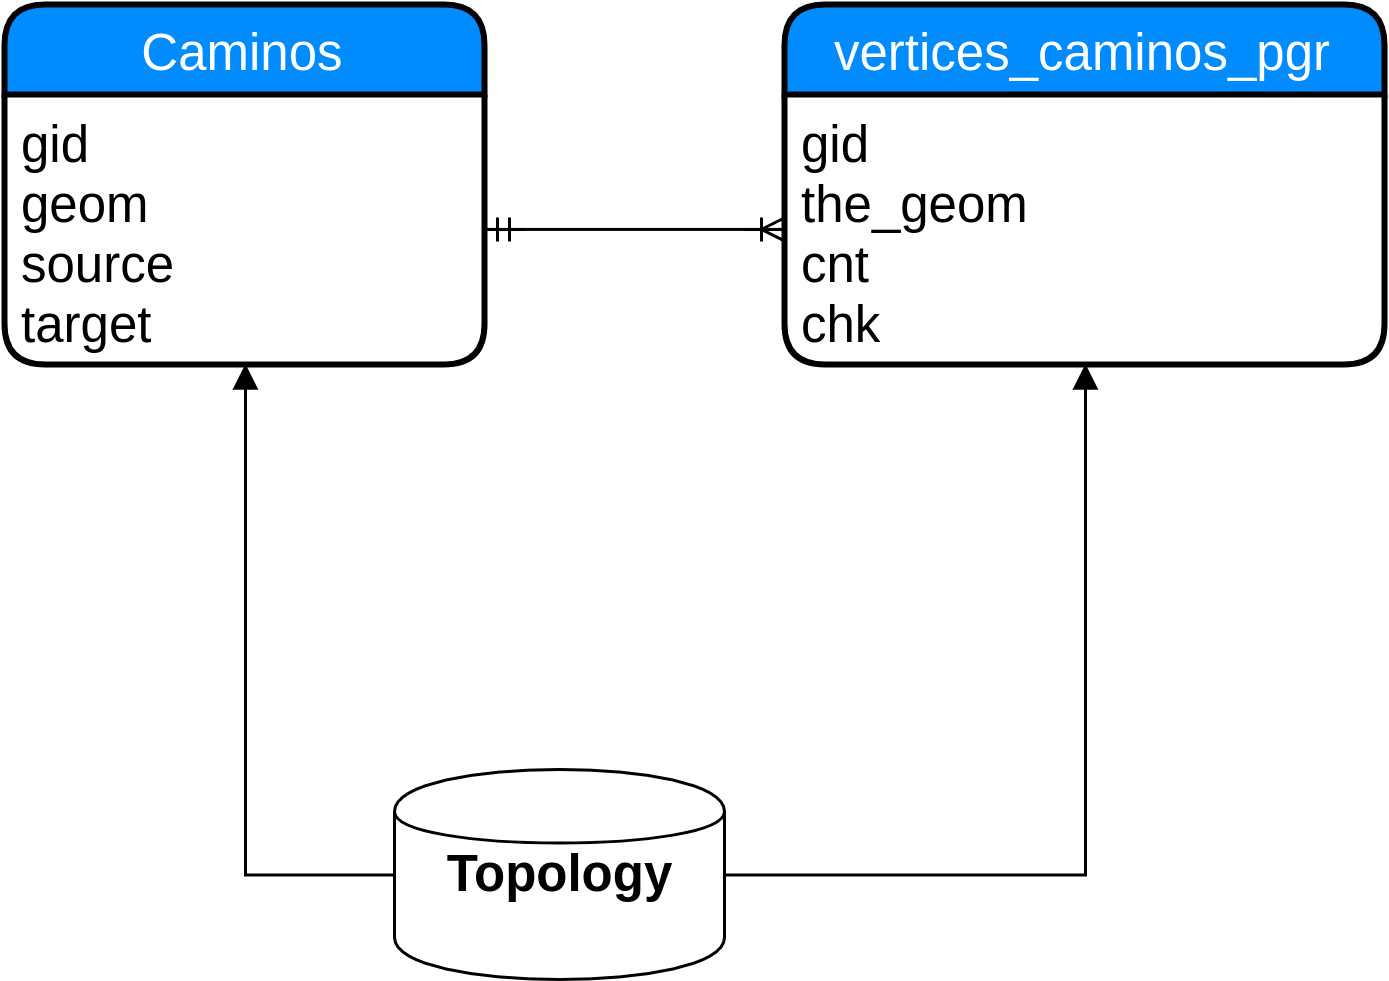
\includegraphics[width=0.4\textwidth]{diagramas/er_ways}
  \end{center}
  \caption{Diagrama ER: Caminos}
  \label{fig:er_ways}
  \caption*{Fuente: Elaboración propia}
\end{figure}



\item \textbf{Diagrama de Secuencia:}

En la figura \ref{fig:sequence_ruta_optima}, se observa el diagrama de secuencia correspondiente obtención de la ruta óptima.


\begin{figure}[H]
  \begin{center}
    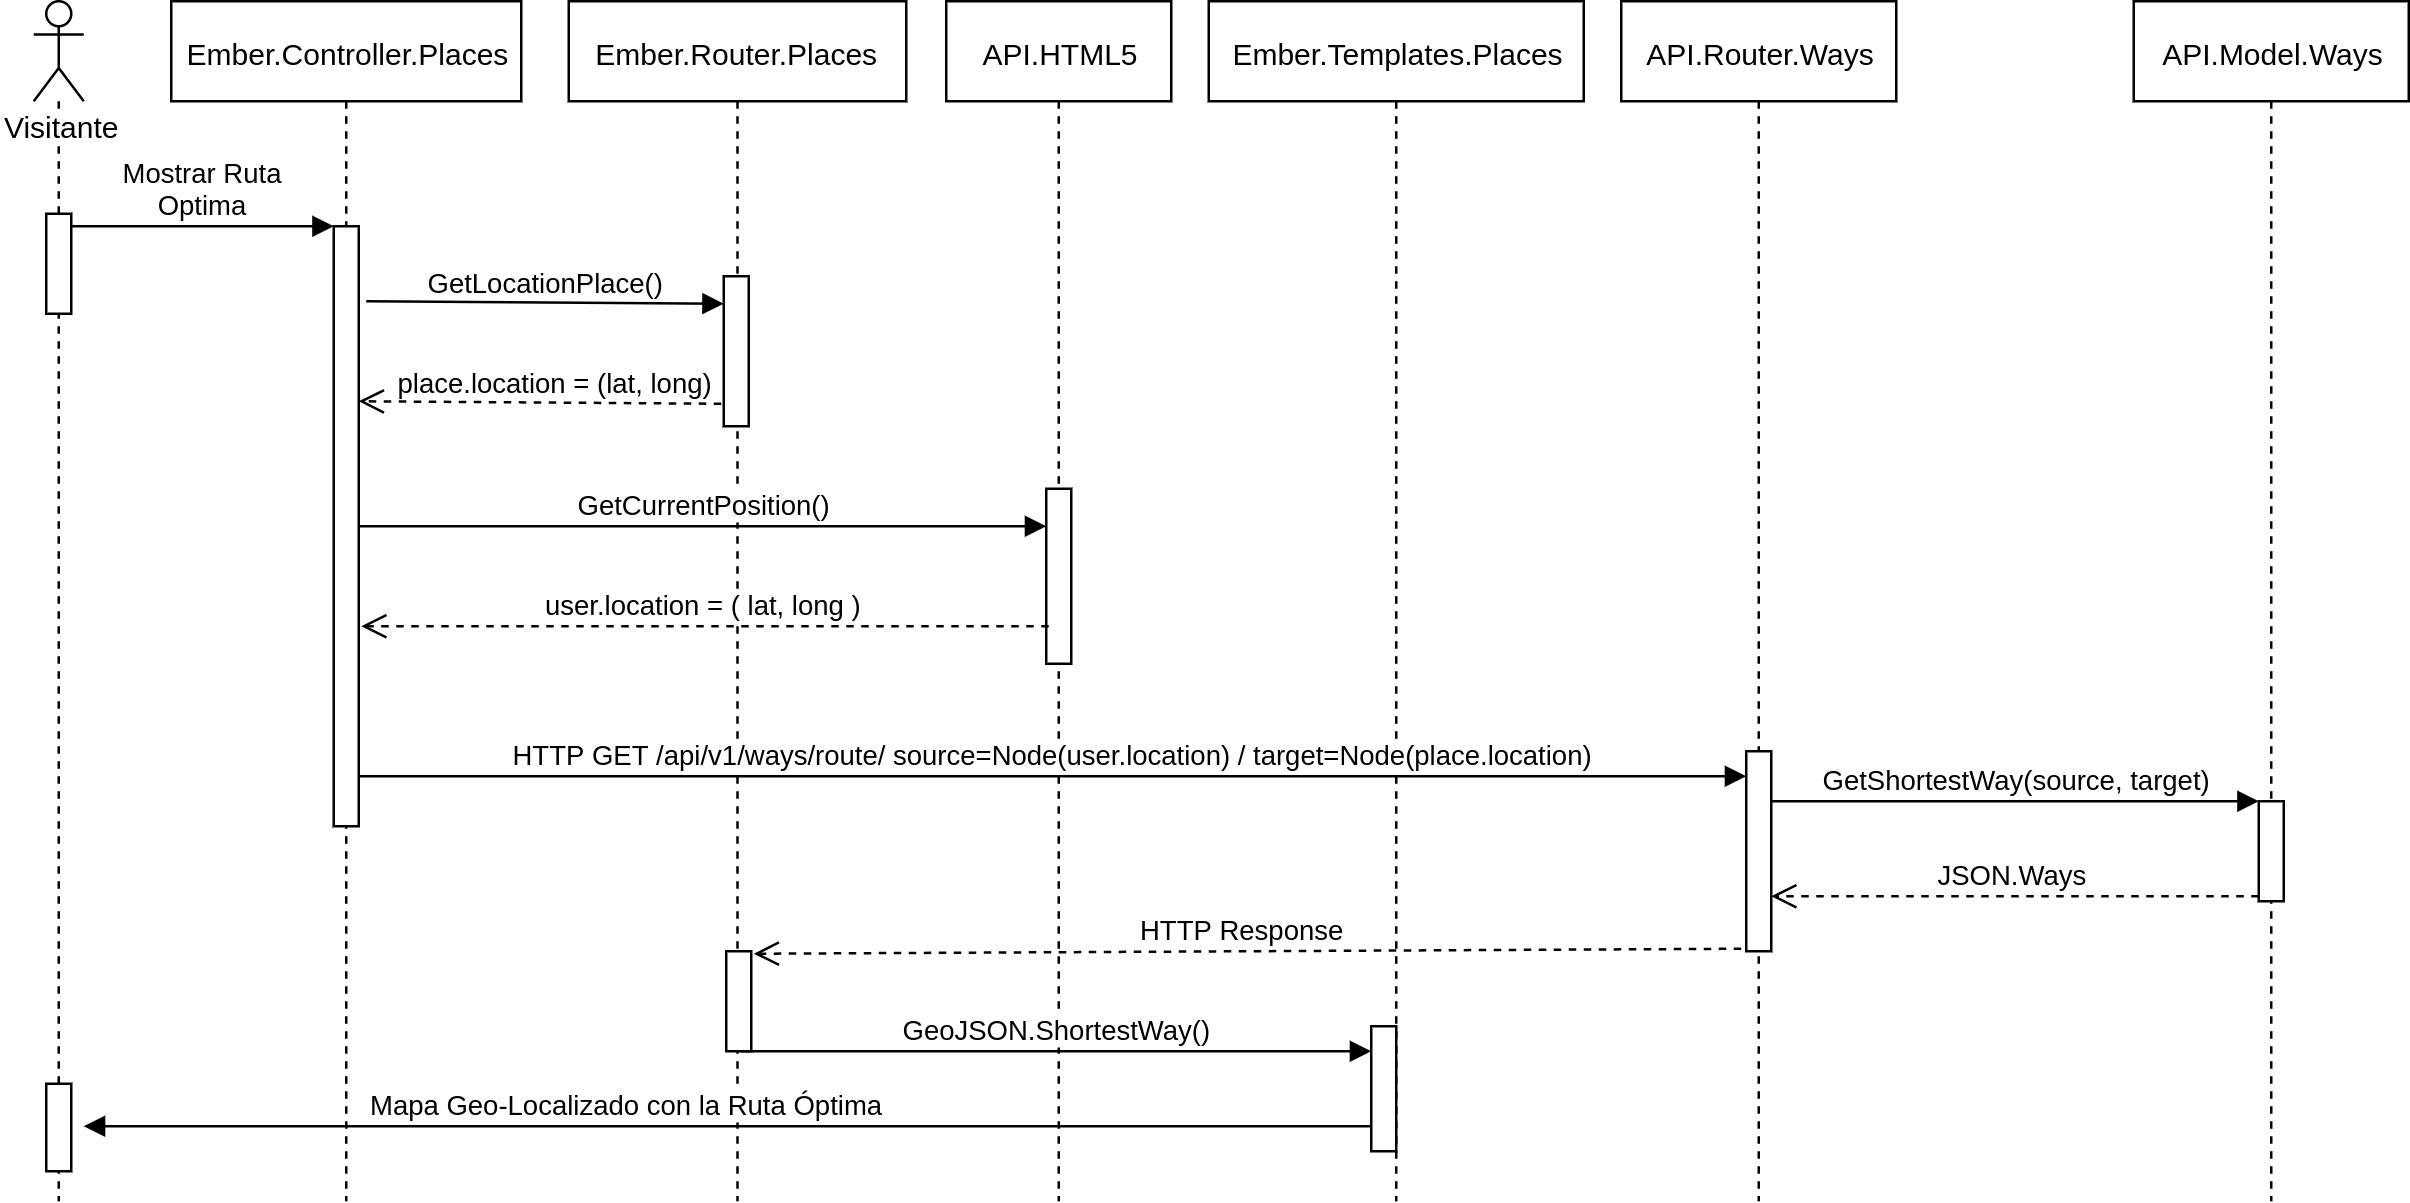
\includegraphics[width=0.9\textwidth]{diagramas/sequence_ruta_optima}
  \end{center}
  \caption{Diagrama de Secuencia: Ruta Óptima}
  \label{fig:sequence_ruta_optima}
  \caption*{Fuente: Elaboración propia}
\end{figure}






\item \textbf{Diagrama de Clases:}

En la figura \ref{fig:clases_caminos}, se observa el diagrama de clases correspondiente a los caminos del campus Universitario.

\begin{figure}[H]
\begin{center}
  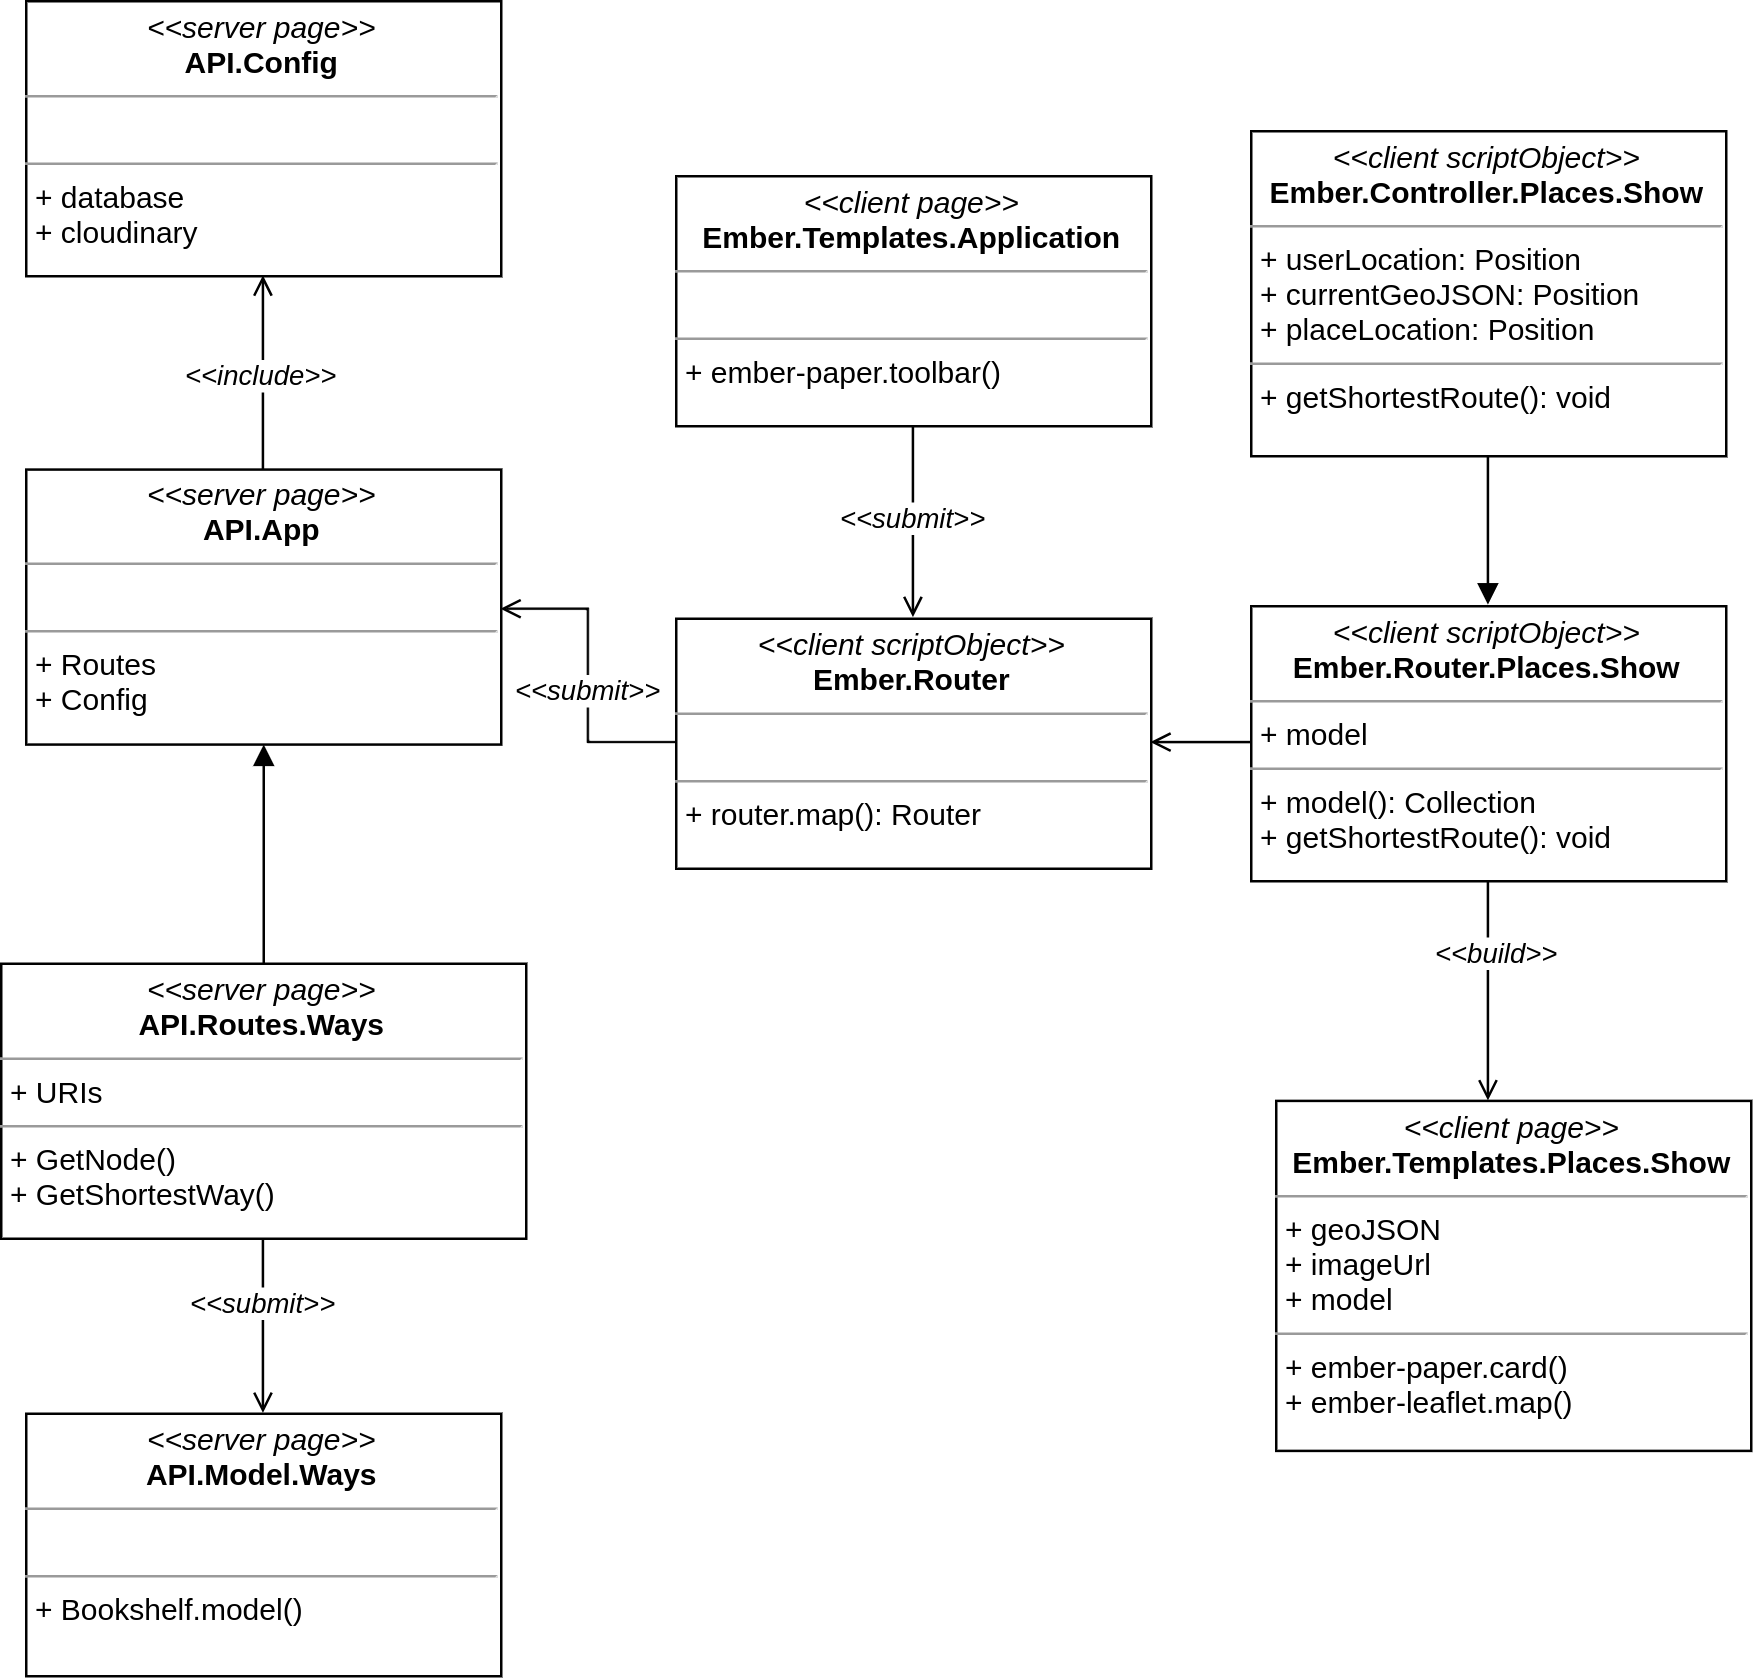
\includegraphics[width=0.9\textwidth]{diagramas/clases_caminos}
\end{center}
\caption{Diagrama de Clases: Caminos}
\label{fig:clases_caminos}
\caption*{Fuente: Elaboración propia}
\end{figure}


\end{itemize}
